\chapter{Background e Stato dell'Arte}

L'evoluzione del panorama delle minacce informatiche ha reso indispensabile lo sviluppo di tecniche e strumenti sempre più sofisticati per l'analisi forense digitale. Questo capitolo fornisce le basi teoriche necessarie per comprendere il contesto in cui si inserisce il presente lavoro, esplorando i concetti fondamentali del Digital Forensics and Incident Response (DFIR), con particolare attenzione all'analisi della memoria volatile. Verranno inoltre esaminati i principali framework esistenti, con focus su Volatility e YARA, evidenziando le limitazioni che motivano le espansioni proposte in questa tesi.

\section{Digital Forensics e Incident Response (DFIR)}

\subsection{Definizione e principi fondamentali}

Il Digital Forensics and Incident Response (DFIR) rappresenta la convergenza di due discipline complementari che, insieme, formano il nucleo delle capacità di risposta alle minacce cyber moderne. Il termine DFIR è stato coniato per riflettere la natura interconnessa di queste attività nel contesto operativo reale.

La \textbf{Digital Forensics} è definita dal NIST come "l'applicazione di scienza e metodi per identificare, preservare, raccogliere, validare, analizzare, interpretare, documentare e presentare evidenze digitali derivate da fonti digitali allo scopo di facilitare o promuovere la ricostruzione di eventi" \cite{kent2006}. Questa disciplina si basa su quattro principi scientifici fondamentali: la \textbf{preservazione dell'evidenza} per garantire che i dati non vengano alterati durante l'acquisizione e l'analisi; la \textbf{chain of custody} che documenta ogni passaggio per mantenere l'ammissibilità legale; la \textbf{ripetibilità} delle analisi che devono produrre risultati consistenti; e la \textbf{documentazione completa} dove ogni azione deve essere registrata e giustificata.

Questi principi sono ulteriormente codificati negli standard internazionali come ISO/IEC 27037:2012 \cite{iso27037}, che fornisce linee guida per l'identificazione, raccolta, acquisizione e preservazione delle evidenze digitali, enfatizzando rilevanza, affidabilità, sufficienza e conformità alle normative locali. Similmente, le linee guida SWGDE \cite{swgde2022} stabiliscono best practices specifiche per la preservazione di evidenze volatili come pagine web, social media e comunicazioni cloud-based.

L'\textbf{Incident Response} si concentra invece sulla gestione operativa degli incidenti di sicurezza con l'obiettivo di minimizzare l'impatto e ripristinare le operazioni normali nel minor tempo possibile. Il SANS Institute la definisce come "un approccio organizzato per affrontare e gestire le conseguenze di una violazione della sicurezza o di un attacco informatico" \cite{sans2023}.

La fusione di queste discipline nel DFIR riconosce che, nel mondo reale, l'analisi forense e la risposta agli incidenti sono attività inseparabili. Durante un incidente attivo, i responder devono bilanciare molteplici esigenze contrastanti: contenere la minaccia mentre preservano le evidenze, analizzare i sistemi compromessi senza interrompere le operazioni critiche, e trovare il giusto equilibrio tra la necessità di un'indagine approfondita e l'urgenza del ripristino operativo.

\subsection{Il processo DFIR}

Il processo DFIR segue un approccio metodologico articolato in sei fasi distinte, come definito dal framework NIST SP 800-61 \cite{cichonski2012}. Sebbene questa struttura fornisca un modello logico di riferimento, nella pratica operativa le fasi si sovrappongono frequentemente e richiedono un approccio iterativo.

\begin{figure}[H]
    \centering
    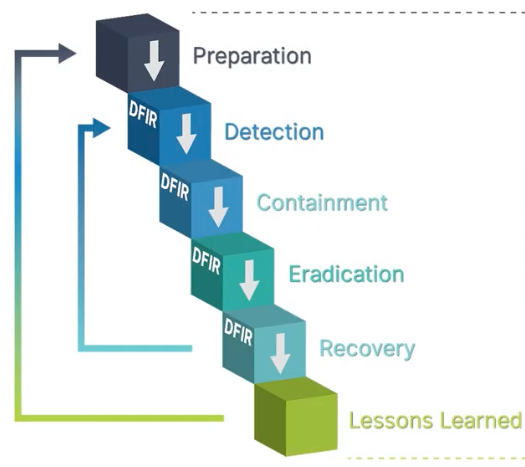
\includegraphics[width=0.6\linewidth]{images/stato-arte/digital-forensics-incident-response-plan-flow.png}
\end{figure}

La \textbf{preparazione} rappresenta il fondamento dell'intero processo, determinando la differenza tra una risposta efficace e una gestione caotica. Questa fase richiede lo sviluppo preventivo di playbook e procedure operative standard, supportati da un'infrastruttura tecnologica adeguata e training continuo del personale.

L'\textbf{identificazione} inizia con l'analisi degli alert provenienti dai sistemi di sicurezza, seguita da un processo di triage che distingue i falsi positivi dalle minacce concrete. Il \textbf{contenimento} diventa poi prioritario per limitare la propagazione del danno attraverso azioni immediate di isolamento e misure sostenibili a lungo termine, sempre preservando le evidenze forensi.

L'\textbf{eradicazione} richiede un approccio sistematico che va oltre la rimozione degli artefatti visibili, identificando tutti i componenti malevoli, incluse backdoor e meccanismi di persistenza nascosti. Il \textbf{recupero} rappresenta una fase delicata dove la ricostruzione deve partire da backup verificati, accompagnata da monitoraggio intensificato. Infine, la fase di \textbf{lessons learned} trasforma ogni incidente in un'opportunità di miglioramento attraverso documentazione dettagliata e analisi critica.

Il DFIR è ormai essenziale nella cybersecurity moderna sia per fronteggiare minacce avanzate come APT e ransomware, sia per rispondere a requisiti normativi stringenti come il GDPR \cite{gdpr2016} che impone notifica entro 72 ore, la direttiva NIS2 \cite{nis2_2022} per operatori essenziali, e il DORA \cite{dora2022} per il settore finanziario. Con il tempo medio di permanenza degli attaccanti sceso a 16 giorni \cite{mandiant2023}, la capacità di risposta rapida ed efficace diventa critica.

\section{Memory Forensics}

\subsection{La memoria volatile come fonte di evidenze}

La memoria volatile, principalmente la RAM, rappresenta lo stato "vivo" di un sistema informatico catturando informazioni effimere ma fondamentali che rivelano con precisione cosa stava accadendo al momento dell'acquisizione \cite{ligh2014}. A differenza dello storage persistente, la memoria offre una finestra unica sui processi in esecuzione, le connessioni di rete attive, e i dati temporaneamente decifrati.

L'architettura della memoria segue una gerarchia complessa: dai registri CPU ultra-veloci ma minuscoli, attraverso le cache L1-L3 progressivamente più capienti, fino alla RAM principale che costituisce l'area di lavoro del sistema. Questa contiene lo \textit{spazio kernel} con le strutture critiche del sistema operativo, lo \textit{spazio utente} dove risiedono processi e applicazioni, la \textit{pool memory} per allocazioni dinamiche, e la \textit{page cache} con i dati dei file recenti.

La gestione della memoria virtuale aggiunge complessità ma anche opportunità investigative. Ogni processo opera in uno spazio di indirizzamento isolato, con pagine virtuali mappate dinamicamente su frame fisici attraverso page tables e translation lookaside buffers. Per l'analista forense, ricostruire questi mapping è essenziale per interpretare correttamente il contenuto della memoria \cite{case2017}.

\subsection{Artefatti recuperabili e vantaggi dell'analisi}

La memoria volatile conserva artefatti unici non reperibili altrove. I \textbf{processi e thread} rivelano l'intera lista dei processi, inclusi quelli nascosti da rootkit, con argomenti command line, variabili d'ambiente, handle aperti, stack e heap contenenti tracce dell'esecuzione. Le \textbf{informazioni di rete} mostrano connessioni TCP/UDP attive, socket in ascolto che potrebbero nascondere backdoor, cache DNS e buffer di pacchetti.

Particolarmente critici sono gli \textbf{artefatti di sicurezza}: token di autenticazione e chiavi crittografiche temporaneamente in chiaro, certificati SSL/TLS, ticket Kerberos, hash NTLM e password di applicazioni. Le \textbf{evidenze di malware} includono codice iniettato in processi legittimi, API hooks, driver kernel malevoli, payload cifrati decriptati solo a runtime, e comunicazioni C\&C. Le \textbf{tracce di attività utente} comprendono clipboard, titoli di finestre, cronologia comandi, documenti in editing e chat in chiaro.

L'analisi della memoria offre vantaggi unici rispetto all'analisi del disco. Garantisce visibilità su minacce fileless e tecniche living-off-the-land che non lasciano tracce su disco. Permette l'accesso a dati normalmente cifrati, osservabili in chiaro durante l'esecuzione. Fornisce una visione runtime completa con processi, connessioni e allocazioni dinamiche, con una timeline difficilmente falsificabile. Inoltre, bypassa molte contromisure anti-forensi poiché modifiche ai file o cancellazioni secure non influenzano le strutture in RAM.

\section{Framework e Strumenti per l'Analisi della Memoria}

\subsection{Volatility Framework}

Volatility \cite{volatility2024} rappresenta lo standard de facto per l'analisi forense della memoria dal suo rilascio nel 2007. Creato inizialmente da Aaron Walters per democratizzare l'accesso a tecniche precedentemente riservate a poche agenzie, il framework si è evoluto attraverso tre versioni maggiori. Volatility 2.0 (2011) introdusse l'architettura plugin-based che ne permise l'espansione da parte della community. Volatility 3 (2019) rappresentò una riscrittura completa in Python 3, risolvendo limitazioni architetturali accumulate e migliorando significativamente le performance.

L'architettura di Volatility 3 si basa su componenti modulari elegantemente integrati. Il \textbf{Framework Core} orchestra configurazione ed esecuzione, mentre le \textbf{Symbol Tables} permettono di interpretare le strutture dati specifiche di ogni versione di sistema operativo. Gli \textbf{Address Spaces} forniscono astrazione per diversi formati di dump, i \textbf{Plugins} implementano la logica di estrazione degli artefatti, e i \textbf{Renderers} gestiscono l'output in formati multipli.

Il framework offre oltre 100 plugin che coprono ogni aspetto dell'analisi. Per l'analisi dei processi, \texttt{pstree} visualizza relazioni gerarchiche evidenziando anomalie parent-child spesso indicative di injection, mentre \texttt{psscan} esegue scansioni euristiche per scoprire processi nascosti da rootkit. L'estrazione delle command line con \texttt{cmdline} rivela gli obiettivi degli attaccanti, e l'analisi di DLL e handle fornisce insight sulle risorse manipolate.

Per l'analisi di rete, \texttt{netscan} (ottimizzato per Windows Vista+) fornisce una visione comprensiva delle connessioni, evoluzione dei precedenti plugin per sistemi legacy. La detection di malware si avvale di \texttt{malfind} che implementa euristiche sofisticate per identificare code injection cercando pagine eseguibili non mappate a file - combinazione altamente sospetta. Plugin complementari come \texttt{hollowfind} specializzano la ricerca verso process hollowing, mentre l'analisi dei callback kernel può rivelare rootkit a livello kernel.

Nonostante la sua potenza, Volatility presenta limitazioni significative. L'interfaccia command-line risulta intimidatoria per utenti meno tecnici, e interpretare correttamente l'output richiede profonda conoscenza delle strutture OS. L'output testuale necessita di post-processing intensivo, non esiste automazione built-in per workflow comuni, e manca gestione integrata di casi multipli - problematica in investigazioni che coinvolgono decine di sistemi.

\subsection{Pattern Matching con YARA}

YARA \cite{yara2024}, creato da Victor M. Alvarez presso VirusTotal nel 2008, è diventato lo standard per pattern matching e classificazione di malware. Il suo successo deriva dalla capacità di descrivere famiglie di malware attraverso regole basate su caratteristiche testuali o binarie, applicabili a file, processi o dump di memoria.

La sintassi YARA bilancia espressività e semplicità. Una regola tipica contiene tre sezioni: \textbf{meta} con metadati descrittivi, \textbf{strings} che definisce i pattern da cercare (stringhe, hex, regex), e \textbf{condition} che specifica la logica booleana per il matching. 

\begin{minted}[
    breaklines,
    frame=lines,
    framesep=2mm,
    baselinestretch=1.2,
    fontsize=\small,
    linenos
]{c}
rule ExampleRule {
    meta:
        author = "Security Researcher"
        description = "Detects Example Malware"
        date = "2024-01-01" 
    strings:
        $text_string = "malicious_function"
        $hex_string = { 6A 40 68 00 30 00 00 6A 14 8D }
        $regex = /\w+\.exe/
    condition:
        any of them
}
\end{minted}

La flessibilità delle condizioni permette logiche detection estremamente sofisticate utilizzando operatori logici, contatori, offset e funzioni built-in. Le condizioni possono essere semplici ("any of them") o complesse, combinando multipli criteri per ridurre i falsi positivi e aumentare l'accuratezza del rilevamento.

Quando applicato alla memoria, YARA trasforma le capacità investigative. Eccelle nell'identificare malware che esistono solo runtime - shellcode iniettato in processi legittimi, DLL reflective che non toccano disco, payload che si materializzano solo post-exploitation. Durante il threat hunting, YARA cerca stringhe uniche di famiglie malware specifiche, pattern di comunicazione C2, o artefatti di tool post-exploitation come Cobalt Strike.

La vera potenza emerge nel rilevamento di tecniche di evasione. YARA può identificare pattern lasciati da process hollowing dove processi legittimi vengono svuotati e riempiti con codice malevolo, riconoscere API hooks sospetti, o pattern di allocazione memoria che tradiscono injection avanzate. Ogni tecnica di evasione, per quanto sofisticata, lascia inevitabilmente una firma che YARA può essere addestrata a riconoscere.

Volatility integra nativamente YARA attraverso il plugin \texttt{yarascan}, che non si limita a segnalare match ma fornisce ricco contesto forense: offset di memoria per correlazioni, processo proprietario per attribuzione, permessi della pagina (RWX spesso indica injection), e dump del contenuto circostante per analisi manuale approfondita.

I vantaggi di YARA nella memory forensics includono standardizzazione attraverso un linguaggio comune per descrivere pattern, flessibilità nel definire condizioni detection complesse mantenendo leggibilità, performance ottimizzate per scansioni rapide su grandi volumi, manutenibilità con regole versionabili in repository condivisi, e portabilità delle stesse regole applicabili a file, memoria o traffico di rete.

Esistono tuttavia sfide nell'uso di YARA per l'analisi della memoria. La frammentazione della memoria virtuale può spezzare pattern su pagine non contigue. Pattern troppo generici generano falsi positivi in ambienti con molti processi. Malware evoluti usano cifratura, offuscamento e polimorfismo per evadere il pattern matching statico. Le scansioni di dump molto grandi con ruleset estesi possono richiedere tempo significativo. Infine, mantenere regole aggiornate richiede effort continuo data l'evoluzione costante delle minacce.

\subsection{Limitazioni degli approcci attuali}

Nonostante la maturità degli strumenti disponibili, l'adozione della memory forensics rimane limitata da barriere sistemiche che ne impediscono il pieno potenziale.

La \textbf{complessità tecnica} costituisce l'ostacolo principale. L'analisi efficace richiede non solo competenza sui tool ma comprensione profonda di architetture OS, gestione memoria, e tecniche anti-forensics. Interpretare i risultati necessita esperienza per distinguere comportamenti normali da anomalie in contesti diversi. La necessità di scripting per automazione esclude personale non programmatore, creando un collo di bottiglia nelle capacità investigative delle organizzazioni.

La \textbf{mancanza di standardizzazione} dell'industria risulta in formati output incompatibili tra tool, impossibilità di condividere risultati tra team con stack diversi, e requirement di sviluppo custom per ogni integrazione SIEM/SOAR. Workflow e procedure variano drasticamente tra organizzazioni, complicando training e collaborazione.

I problemi di \textbf{scalabilità} emergono in scenari enterprise dove incidenti coinvolgono centinaia di endpoint. L'analisi sequenziale di dump multipli (spesso 100GB+ ciascuno) diventa proibitiva. La mancanza di parallelizzazione nativa e la correlazione manuale tra findings di sistemi diversi introducono inefficienze critiche in contesti time-sensitive.

L'\textbf{user experience inadeguata} allontana utenti abituati a interfacce moderne. Output testuali densi senza visualizzazioni rendono difficile identificare pattern. Generare report per management richiede ore di formatting manuale. La collaborazione è complicata da formati proprietari e mancanza di workspace condivisi.

L'\textbf{integrazione limitata} con l'ecosistema di sicurezza riduce il valore operativo. Threat intelligence feeds non si integrano nativamente, la correlazione con logs e network traffic è manuale, export verso piattaforme avanzate richiede trasformazioni complesse, e API limitate impediscono automazione enterprise-grade.

Queste limitazioni creano un gap sostanziale tra il valore teorico della memory forensics e la sua applicazione pratica. In contesti ad alta pressione come incident response real-time o cyber defense exercises tipo Locked Shields, queste inefficienze possono determinare il successo o il fallimento dell'investigazione. È proprio per colmare questo gap che nascono piattaforme come VolWeb \cite{volweb2024}, progettate per democratizzare l'accesso alla memory forensics attraverso interfacce intuitive e automazioni intelligenti.